% =====================================================================
%  Schematic summary of the project: experiments, designs tried, and
%  short notes on what seems to work, in two parts: Part I, the identification
%  strategy on the simple tasks; Part II, the complex tasks. Kept up to date with each new
%  experiment or design change; the full text is proposal-minimal.tex.
% =====================================================================
\documentclass[10pt,a4paper]{article}

\usepackage[utf8]{inputenc}
\usepackage[T1]{fontenc}
\usepackage[margin=1.8cm]{geometry}
\usepackage{amsmath,amssymb}
\usepackage{booktabs,tabularx,array}
\usepackage{enumitem}
\usepackage{pifont}
\usepackage{xcolor}
\usepackage{xltabular}
\usepackage{tikz}
\usetikzlibrary{positioning,arrows.meta}
\usepackage[colorlinks=true,linkcolor=blue!50!black,urlcolor=blue!60!black]{hyperref}

\setlist{nosep,leftmargin=*}
\setlength{\parindent}{0pt}
\setlength{\parskip}{4pt}
\renewcommand{\arraystretch}{1.15}
\newcolumntype{L}{>{\raggedright\arraybackslash}X}

% Verdict marks
\newcommand{\yes}{\textcolor{green!45!black}{\ding{51}}}
\newcommand{\no}{\textcolor{red!70!black}{\ding{55}}}
\newcommand{\mixed}{\textcolor{orange!80!black}{$\sim$}}

\title{Lexical Task Heads beyond Simple Tasks\\\large Schematic project summary}
\author{Filippo Merlo}
\date{Last updated: 3 November 2026}

\begin{document}
\maketitle
\vspace{-1em}

\noindent Marks: \yes{} works / supports the hypothesis, \no{} does not, \mixed{} mixed or task-dependent. Full methods and tables: \texttt{proposal-minimal.tex}.

\noindent The project has two parts. \textbf{Part I} works on the lexical-head identification strategy on the simple tasks (current focus); \textbf{Part II} tries it on the complex tasks. Section~\ref{sec:setup} is shared.

% ---------------------------------------------------------------------
\section{Setup in one page (both parts)}\label{sec:setup}

\begin{tabularx}{\textwidth}{@{}>{\raggedright\arraybackslash\bfseries}p{2.8cm}L@{}}
\toprule
Part I question & Does the lexical-task-head method of Yang et al.\ (2026) reproduce on our setup, does Head-JLens (J-head) find heads the per-head logit lens (Logit-head) misses, and which heads should be kept when a task is asked for in several wordings? Simple tasks. \\
Part II question & Does the method find task-carrying heads on the complex, rule-defined tasks of Fu et al.\ (2026), under either readout? \\
Model & Llama-3.1-8B-Instruct (bf16; only model with released Head-JLens matrices). \\
Readouts & Logit-head: head write $c_{l,h}$ decoded by the unembedding. J-head: head output $z_{l,h}$ mapped through the fitted Jacobian $J_{l,h}$, then decoded. \\
Simple tasks & 14 Todd et al.\ tasks (antonym, capitals, translation, \dots). Rule style: 5 instruction templates; example style: 1/5/10/20/30 shots; zero-shot prompt. Raw text, no chat template. \\
Complex tasks & Fu et al.'s 5 tasks, easy level: Set Game, Tapatan, Operator Function, Noun Class Agreement (NCA), Lexical Category Inference (LCI). 300 items (LCI 600). Rule style: original + 6 GPT-5.5 wordings; example; combined; input block only (no task info). Chat template, greedy, up to 1,024 tokens. \\
Head criterion & Head is a lexical task head on a prompt if $\geq 1$ of its top-10 tokens is in the task's term list; for the style if this holds on $\geq 10\%$ of $P^+$ (first 100 correct prompts of the most accurate wording). \\
Term lists & Simple: Yang et al.'s (2--22 token ids). Complex: GPT-5.5, checked by hand (114--340 token ids). \\
Causal check 1 & Yang App.~G.1: patch the mean head output ($\times\alpha$) at the last token of prompts \emph{without} task info; control = mean of another task at the same heads. \\
Causal check 2 & Yang's released script: patch prompts that \emph{give} the task but were answered wrongly (baseline 0). Complex tasks: control added. \\
Head sets patched & $H^L$, $H^J$, and J-only $H^J\setminus H^L$. \\
\bottomrule
\end{tabularx}

\medskip
\begin{center}
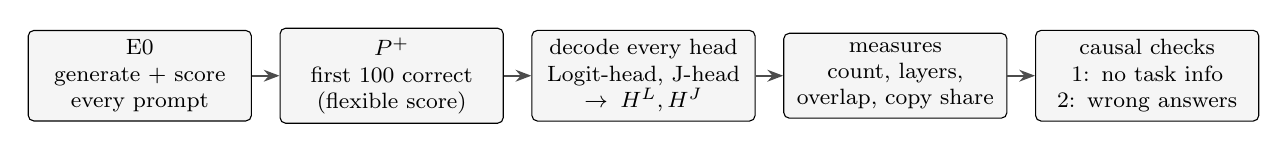
\begin{tikzpicture}[
  node distance=4mm and 3.5mm,
  box/.style={draw, rounded corners=2pt, fill=gray!8, align=center, font=\footnotesize, minimum height=9mm, text width=2.6cm},
  arr/.style={-{Stealth[length=2mm]}, thick, gray!60!black}]
\node[box] (e0) {E0\\generate + score\\every prompt};
\node[box, right=of e0] (p) {$P^{+}$\\first 100 correct\\(flexible score)};
\node[box, right=of p] (h) {decode every head\\Logit-head, J-head\\$\to H^L, H^J$};
\node[box, right=of h] (m) {measures\\count, layers,\\overlap, copy share};
\node[box, right=of m] (c) {causal checks\\1: no task info\\2: wrong answers};
\draw[arr] (e0) -- (p); \draw[arr] (p) -- (h); \draw[arr] (h) -- (m); \draw[arr] (m) -- (c);
\end{tikzpicture}
\end{center}

\medskip
\textbf{Design changes for both parts}

\small
\begin{tabularx}{\textwidth}{@{}p{1.5cm}LLL@{}}
\toprule
\textbf{Date} & \textbf{Tried first} & \textbf{Replaced by} & \textbf{Why / effect} \\
\midrule
10-27 & Rules as main style, examples secondary & Rule and example treated alike & No main condition (user decision). \\
10-28 & Prompts and means pooled over wordings & One wording for heads, one mean per wording (Yang's code) & Matches the source exactly. \\
10-28 & Check 1 only (zero-shot) & Check 1 + check 2 (released script) & Only check 2 reproduces Yang's figures. \\
10-30 & First-token (simple) / strict (complex) score for heads and checks & Flexible score; E1, E2 rerun & Strict scoring created spurious wording differences. \\
\bottomrule
\end{tabularx}
\normalsize

\medskip
\textbf{Across both parts}
\begin{itemize}
\item \yes{} \textbf{Scoring matters first.} Flexible scoring removes most of the apparent wording sensitivity; always check it before reading wording effects.
\end{itemize}

% =====================================================================
\section{Part I --- identification strategy on simple tasks}\label{sec:part1}

\subsection{Experiments and outcomes}
\small
\begin{xltabular}{\textwidth}{@{}>{\raggedright\arraybackslash}p{2.5cm}>{\hsize=.8\hsize}L>{\hsize=1.2\hsize}Lc@{}}
\toprule
\textbf{Experiment} & \textbf{Design} & \textbf{Outcome (short)} & \\
\midrule
\endhead
\multicolumn{4}{@{}l}{\textbf{E0 --- behavioural baseline (simple tasks)}} \\
Simple tasks & 14 tasks $\times$ 11 prompts, every item. & All tasks well above zero-shot; accuracy rises 1$\to$5 shots then flat. Template spread largest on translation, next/prev-item, park--country, synonym. & \yes \\
Scoring audit & Every reply saved; strict (first token) vs flexible vs GPT-5.5 judge; disagreement reasons. & Translation spread mostly quotes/capitals; first-token score marks any number correct. & \yes \\
\midrule
\multicolumn{4}{@{}l}{\textbf{E1 --- simple tasks} (14 tasks $\times$ rule/example $\times$ 2 readouts)} \\
Head sets & 100 prompts per style; most accurate template / 5-shot. & Logit-head finds heads on every task. J-head finds more on 23/28 pairs; its extra heads sit in layers 10--19 (Logit-head mostly $\geq$20). J-head contains all of Logit-head only on 4/28. Example heads mostly inside rule heads. & \yes \\
Check 1 (zero-shot) & Means per wording, 15 $\alpha$ values, control mean. & Logit-head: gain $\geq$10 items on capitals, landmark, park, product (+ currency, next-item, plural with examples). Nothing on antonym, synonym, present--past, prev-item, translations. Best around $\alpha=4$. Control mostly low (not on park--country, next-item). & \mixed \\
Check 1, J-head & same & J-head $\geq$ Logit-head on most tasks; J-only heads have effects of their own. & \yes \\
Cross-style means & Rule heads $\times$ example means and vice versa. & Same tasks gain, often as much or more. & \yes \\
Check 2 (1-shot wrong) & Yang's released script, no control. & Gains on all 14 tasks; reproduces Yang's Figs.~57/62 task order. J-head far stronger on next/prev-item with examples. & \yes \\
\midrule
\multicolumn{4}{@{}l}{\textbf{E1b --- heads from several templates} (rule style, simple tasks)} \\
$k=5$ (all templates) & Heads passing under all 5 templates; both checks. & Better on fact tasks (capitals, park, product) only; worse elsewhere. Beats E1 on $\leq$4/14 tasks. & \no \\
$k=1$ (union) & Exploratory. & Helps J-head on present--past (0$\to$16 items), synonym, prev-item, control flat. Hurts Logit-head on fact tasks. & \mixed \\
$k=3$ & Exploratory. & Mostly the E1 heads; behaves like E1. & -- \\
$k=1$, shared & J-head union, kept only heads in the union sets of $\geq 2$ tasks (keeps 15--62 of 19--74 heads per task); both checks. & \textbf{Not successful.} Removes most of the union's gains: present--past 16$\to$1 items (check 1), 0.64$\to$0.45 (check 2); synonym 0.21$\to$0.13. Only country--capital rises (0.60$\to$0.69). Shared heads do not carry the task better. & \no \\
$k=1$, 4 present--past heads & The 4 heads only present--past's union set contains (L19H10, L19H24, L20H28, L21H9; none in E1); both checks, present--past only. & Check 1: no effect alone (0.01); needs the other 15 heads too. Check 2: 0.63, as the whole 19-head union (0.64); rises with $\alpha$ up to 10, real past forms (60/61 distinct replies); $\alpha=0$ gives 0.02. & \mixed \\
Replies, present--past & Each patched reply sorted by kind, per head set and $\alpha$ (J-head, rule means; notebook below). & Shared heads make the model \emph{name} the task (``past tense of assess'': 65\% of replies in check 1, 73\% in check 2 at $\alpha=10$) without doing it. The 4 unshared heads make it give \emph{a form of the input}: from a bare prompt it repeats the verb (44\%), when the prompt shows the task they fix the inflection. Together (union) they give the answer. One task; heuristic reply kinds. & -- \\
Replies, all tasks & Same, every task. & Many patched replies contain the expected answer after a prefix the flexible score rejects (``Capital -- Tbilisi'', ``plural needles'', ``Country -- Russia, \dots''): 19--33\% of E1 J-head replies at $\alpha=4$ on capitals, landmark, antonym, synonym, singular--plural. Not all are answers (``opposite of solid'' for \emph{hollow}). & -- \\
Retrieval heads & Yang et al.'s retrieval heads (their code): Definition 1 with the prompt's own answer token as target, on E1's identification prompts; overlap with every lexical set, against layer-matched chance. & Mostly distinct from lexical task heads: 2--9\% of each set's heads are retrieval heads, at chance under Logit-head (0.6--1.2$\times$), slightly above under J-head (1.1--1.7$\times$, highest for $k=5$). None on the translation tasks. Of the 4 present--past unshared heads only L21H9 is one (15\% of prompts). & -- \\
4 heads split & Present--past, both checks: L21H9 (the one retrieval head of the 4) alone, and L19H10, L19H24, L20H28 alone. & L21H9 carries the effect: check 2 0.60 alone (4 heads 0.63, 3 heads 0.24); in check 1 it alone makes the model repeat the verb (44\% at $\alpha=10$), as the 4 heads do, and the 3 heads do nothing. A retrieval head that brings the input word forward; the inflection comes from the prompt's example (check 2) or the shared heads (check 1). & \mixed \\
$k=1$ without retrieval heads & $k=1$ sets (L and J) minus every retrieval head of the task (any template, either readout): 51/389 L and 84/672 J heads removed, none on translations; both checks, all tasks. & Mostly small changes, but task-dependent. Landmark--country collapses (check 1: L 0.72$\to$0.02, J 0.75$\to$0.13; J replies still name the country, not first). Present--past J loses its gains (L21H9 removed). Gains on synonym J (0.21$\to$0.32), product--company J (0.35$\to$0.48, control 0.10) and prev-item J check 2 (0.12$\to$0.45, at $\alpha$ 9--10, no constant answer). Park--country L: control now above task. Unchanged sets reproduce $k=1$ exactly. Broad removal: retrieval heads of E1's template and the same readout only would remove 12 L and 51 J heads. & \mixed \\
\bottomrule
\end{xltabular}
\normalsize

\subsection{Hypotheses}

\begin{tabularx}{\textwidth}{@{}>{\raggedright\arraybackslash}p{3.6cm}Lc@{}}
\toprule
H1 replication & Holds with Yang's released setting (check 2); fails with the procedure their paper describes (check 1: no gain on 7 tasks). & \mixed \\
H2 J-head $\supseteq$ Logit-head & Fails: J-head misses part of the Logit-head set on 24/28 pairs. J-only heads are causal in both checks. & \no \\
H3 all-template heads & Falsified: better on $\leq$4/14 tasks. & \no \\
\bottomrule
\end{tabularx}

\subsection{Design variants tried}

\small
\begin{tabularx}{\textwidth}{@{}p{1.5cm}LLL@{}}
\toprule
\textbf{Date} & \textbf{Tried first} & \textbf{Replaced by} & \textbf{Why / effect} \\
\midrule
10-28 & Yang's batching without attention mask & Padding masked & Model attended to padding. \\
11-02 & E1b with $k=5$ only & $k\in\{1,3,5\}$ & After $k=5$ failed; exploratory. \\
\bottomrule
\end{tabularx}
\normalsize

\textbf{Inspecting replies:} \texttt{notebooks/patching\_outputs.py} (marimo) shows the simple-task patched replies for every manipulation: task, check, procedure (E1, $k=1/3/5$, shared/unshared), readout, head and mean style, mean source and wording, $\alpha$; accuracy, the share of the most common reply, reply kinds, and each item's replies.

\subsection{What seems to work, what does not}

\begin{itemize}
\item \yes{} \textbf{Released-code setting (check 2)} is what reproduces Yang et al.; the paper's zero-shot check works only on fact-like tasks.
\item \yes{} \textbf{J-head on simple tasks:} more heads, earlier layers (10--19), and the added heads carry the task causally. It does not contain the Logit-head set.
\item \mixed{} \textbf{Which heads to keep} depends on the task type: all-template heads for fact tasks, union of templates for morphology-like tasks under J-head.
\item \mixed{} \textbf{Retrieval heads} (heads that already write the answer token) are few among lexical task heads, but some effects rest on them: landmark--country's on its 10, present--past's union gain on L21H9. Elsewhere removing them changes little or helps (synonym, product--company, prev-item under J-head). Entity-answer tasks may be carried by retrieval more than by task heads.
\item \mixed{} \textbf{Two roles on present--past} (one task): heads shared across tasks make the model \emph{name} the task; L21H9 makes it give \emph{a form of the input}. Either alone fails from a bare prompt; with an example in the prompt, L21H9 alone suffices.
\item \textbf{Read the replies, not only accuracy:} 19--33\% of patched replies on several tasks contain the answer after a prefix the flexible score rejects, and part of a ``loss'' can be a format change (landmark--country under J-head). \texttt{notebooks/patching\_outputs.py} shows them.
\end{itemize}

% =====================================================================
\section{Part II --- complex tasks}\label{sec:part2}

\subsection{Experiments and outcomes}
\small
\begin{xltabular}{\textwidth}{@{}>{\raggedright\arraybackslash}p{2.5cm}>{\hsize=.8\hsize}L>{\hsize=1.2\hsize}Lc@{}}
\toprule
\textbf{Experiment} & \textbf{Design} & \textbf{Outcome (short)} & \\
\midrule
\endhead
\multicolumn{4}{@{}l}{\textbf{E0 --- behavioural baseline (complex tasks)}} \\
Complex tasks & 5 tasks $\times$ 10 prompts, 300 items. & NCA, LCI answered straight away, above chance. Set Game, Op.\ Function, Tapatan always reason first. Set Game and Op.\ Function solved from rules, hardly from examples alone. Tapatan near chance everywhere. Set Game solved on 97/300 even without task info. & \mixed \\
Scoring audit & Every reply saved; strict (Fu et al.'s parser) vs flexible vs GPT-5.5 judge; disagreement reasons. & Op.\ Function 0.01--0.99 across wordings $\to$ 1.00 everywhere (missing \texttt{\textbackslash boxed}). & \yes \\
\midrule
\multicolumn{4}{@{}l}{\textbf{E2 --- complex tasks} (5 tasks $\times$ rule/example/combined $\times$ 2 readouts)} \\
Head sets & 100 prompts per style (fewer where few correct). & Heads found for every task and style, but counts not comparable with E1 (term lists 10$\times$ longer; Set Game example $P^+$ = 1 prompt). J-head again larger, layers 10--19; covers 44--91\% of Logit-head. Rule/example overlap 48--94\%. & \mixed \\
Check 1 (no task info) & Rule heads, 7 means, 11 $\alpha$, control of same answer format. & Without task info the model does not attempt the task on 4/5 tasks, and no patch changes this. Set Game: $\leq$+5 items, control as much. & \no \\
Check 2 (rules, wrong) & Rule prompts answered wrongly; control added. & Gains everywhere, but the control matches them. $\alpha=0$ alone fixes 21--23 Set Game items; on Yes/No tasks gains = pushing every answer to one label. & \no \\
\bottomrule
\end{xltabular}
\normalsize

\subsection{Hypotheses}

\begin{tabularx}{\textwidth}{@{}>{\raggedright\arraybackslash}p{3.6cm}Lc@{}}
\toprule
H4 complex $<$ simple & Causal part agrees (no task-specific effect on complex tasks); head-count part untestable (term-list length). & \mixed \\
H5 J-head $\supseteq$ Logit-head & Fails: J-head misses part of the Logit-head set on every pair. J-only heads have no task-specific effect. & \no \\
\bottomrule
\end{tabularx}

\subsection{Design variants tried}

\small
\begin{tabularx}{\textwidth}{@{}p{1.5cm}LLL@{}}
\toprule
\textbf{Date} & \textbf{Tried first} & \textbf{Replaced by} & \textbf{Why / effect} \\
\midrule
10-27 & Drop prompts not answered straight away & Reasoning mode for Set Game, Op.\ Function, Tapatan & They are never answered straight away. \\
10-27 & Wordings/terms via ChatGPT & GPT-5.5 via Azure API, checked by hand & API instead of the chat interface. \\
10-27 & All difficulty levels & Easy level only & User decision. \\
10-27 & Reasoning mode: 10 items, $\alpha\in\{0,1,4,10\}$ & 100 items, 11 $\alpha$ values (10-30) & Same 100 items as the other tasks. \\
10-29 & 6,000-token replies, stop at the answer; direct vs reasoning split & 1,024 tokens for all five complex tasks, one scheme & 4/9,000 replies correct after token 1,024. \\
10-29 & Heads also read at a pre-answer position & Last prompt token only & Dropped with its results. \\
10-30 & Tapatan scored by its first line & First label anywhere & First line is the label in 1/3,000 replies. \\
10-31 & Complex check 2 without control & Control mean added & Zero-ablation and label shifts alone gave gains. \\
\bottomrule
\end{tabularx}
\normalsize

\subsection{What seems to work, what does not}

\begin{itemize}
\item \no{} \textbf{Complex tasks:} heads are found, but no causal check shows a task-specific effect. Prompts without task info elicit no attempt; on wrong-answer prompts, any perturbation (zero, control, label shift) helps as much.
\item \no{} \textbf{Head counts on complex tasks} are not interpretable with long term lists and tiny $P^+$ sets.
\item \textbf{Controls are essential} on long-reasoning and Yes/No tasks: without them, check 2 looked positive.
\end{itemize}

% ---------------------------------------------------------------------
\section{Not pursued}
function vectors, function-specific heads, hidden-state differences (scope, 10-27); fp32 Head-JLens fit ($\approx$136 GPU-h, declined); hand-labelled validation of the judge.

\end{document}
